% Created 2020-07-09 jeu. 20:51
% Intended LaTeX compiler: pdflatex
\documentclass[presentation]{beamer}
\usepackage[utf8]{inputenc}
\usepackage[T1]{fontenc}
\usepackage{graphicx}
\usepackage{grffile}
\usepackage{longtable}
\usepackage{wrapfig}
\usepackage{rotating}
\usepackage[normalem]{ulem}
\usepackage{amsmath}
\usepackage{textcomp}
\usepackage{amssymb}
\usepackage{capt-of}
\usepackage{hyperref}
\usepackage{multirow}
\usepackage{tabularx}
\usepackage{booktabs}
\usepackage{caption}
\usepackage{palatino}
\usepackage{newtxmath}
\usetheme{Boadilla}
\author{Maxime Cochennec}
\date{\today}
\title{Résultats de l'article 1}
\hypersetup{
 pdfauthor={Maxime Cochennec},
 pdftitle={Résultats de l'article 1},
 pdfkeywords={},
 pdfsubject={},
 pdfcreator={Emacs 26.3 (Org mode 9.3.6)}, 
 pdflang={English}}
\begin{document}

\maketitle
\begin{frame}{Outline}
\tableofcontents
\end{frame}



\section{Introduction}
\label{sec:org491c0a8}
\begin{frame}[label={sec:orgd908bc7}]{Flow regimes and instabilities in Hele-Shaw cell}
\begin{itemize}
\item Flow regimes:

\begin{itemize}
\item \alert{continuous stream}

\item drop and/or ganglia flow
\end{itemize}
\end{itemize}

Break-up of the invading fluid by snap-off? 

\begin{itemize}
\item Instabilities:

\begin{itemize}
\item Saffman-Taylor

\item Rayleigh-Plateau (see (b) bellow from \cite{cubaud2008capillary})
\end{itemize}
\end{itemize}

\centering
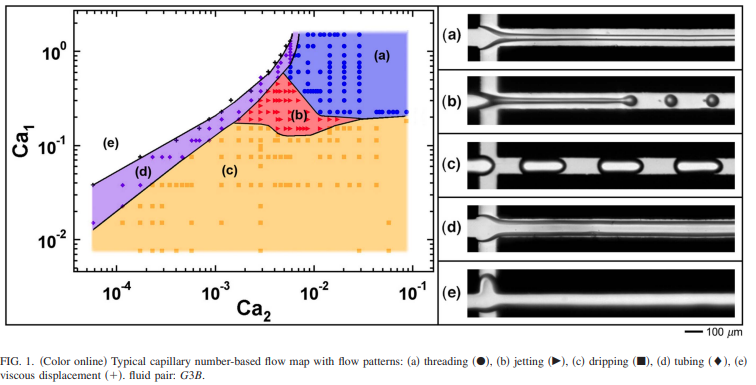
\includegraphics[scale=0.352]{cubaudMason.png}
\end{frame}

\begin{frame}[label={sec:org630fdfe}]{Boundary conditions and simulation parameters}
\begin{table}
\centering{}
\begin{tabular}{cccc}
\toprule 
Boundary & $u$ & $p$ & $\ensuremath{\phi}$\tabularnewline
\midrule
\midrule 
Outlet & - & $0$ & $\mathbf{n}\cdot\boldsymbol{\nabla}\phi=0$\tabularnewline

Inlet $o$ & $u_{o}$ & - & $0$\tabularnewline

Inlet $w$ & $u_{w}$ & - & $1$\tabularnewline
\bottomrule
\end{tabular}\hfill{}%
\begin{tabular}{cc}
\toprule 
Parameters & Value\tabularnewline
\midrule
\midrule 
$Ca=\frac{U_{t}\mu_{o}}{\gamma}$ & from $0.125$ to $0.005$\tabularnewline

$M_{w}=\frac{\mu_{w}}{\mu_{o}}$ & 1\tabularnewline

$f_{f}=\frac{u_{w}}{U_{t}}$ & 1/4\tabularnewline

$h^{*}=h/L$ & from $5$ to $1/20$\tabularnewline
\bottomrule
\end{tabular}
\caption{Boundary conditions (left) and simulation parameters (right)}
\end{table}

\centering
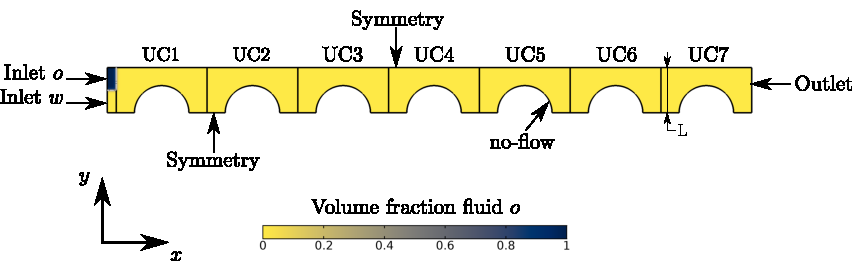
\includegraphics[scale=0.7]{DNS_model.pdf}
\end{frame}

\begin{frame}[label={sec:org1a3e78c}]{Equations}
If \(\nabla \epsilon_i \approx 0\), the momentum transport equations read

\begin{subequations}
\begin{align}
0&=-\varepsilon_{w}\nabla\langle p_{w}\rangle^{w}-\mu_{w}k^{2}\langle\bar{\mathbf{u}}_{w}\rangle+\mathbf{d}_{wc}+\mathbf{d}_{wo},\\
0&=-\varepsilon_{o}\nabla\langle p_{o}\rangle^{o}-\mu_{o}k^{2}\langle\bar{\mathbf{u}}_{o}\rangle+\mathbf{d}_{ow}.
\end{align}
\end{subequations}

where, \(\mathbf{d}_{ij}\) has dimensions \(\mathrm{Pa.m^{-1}}\) i.e. drag forces
per unit surface area (of unit-cell).

\begin{block}{Drag definition}
$\mathbf{d}_{ij}= \frac{1}{S} \int_{\Gamma_{ij}}\sigma_i \cdot \mathbf{n}_{ij} \:
\mathrm{d} \Gamma$, 
\begin{itemize}
\item $\sigma_i$ is the stress-tensor for a Newtonian fluid $i$,
\item $S$ is the unit-cell's surface
\item $\mathbf{n}_{ij}$ is the unit normal vector pointing toward the $j$-phase.
\end{itemize}
\end{block}
\end{frame}
\begin{frame}[label={sec:org20ba60f}]{Drag}
\begin{table}
\begin{centering}
\begin{tabular}{cccc}
\toprule 
\begin{tabular}{c}
Drag of...\tabularnewline
upon...\tabularnewline
\end{tabular} & Fluid $o$ & Fluid $w$ & \tabularnewline
\midrule
\midrule 
Plates & $-\mu_{o}\langle\bar{\mathbf{u}}_{o}\rangle\frac{12}{h^{2}}$ & $-\mu_{w}\langle\bar{\mathbf{u}}_{w}\rangle\frac{12}{h^{2}}$ & \multirow{2}{*}{$\Sigma=\mathbf{d}_{s}$}\tabularnewline
\cmidrule{1-1}
Wedge & - & $\mathbf{d}_{wc}$ & \tabularnewline
\midrule 
Fluid $o$ & - & $\mathbf{d}_{wo}$ & \multirow{2}{*}{$\Sigma=\mathbf{d}_{f}$}\tabularnewline
\cmidrule{1-1} 
Fluid $w$ & $\mathbf{d}_{ow}$ & - & \tabularnewline
\bottomrule
\end{tabular}
\caption{Summary of each drag force terms involved in the averaged momentum
transport equations for two-phase flows in a Hele-Shaw cell.\label{tab:Summary-of-each-drag}}
\par\end{centering}
\end{table}

\begin{alertblock}{Information}
In the following we are interested in the x-component of the drag
(i.e. component align with the main flow direction).
\end{alertblock}
\end{frame}

\section{Results}
\label{sec:org70e6955}

\begin{frame}[label={sec:org11bbfbb}]{Results: flow regimes}
\end{frame}
\begin{frame}[label={sec:orgbf39abd}]{Results: saturation}
\begin{figure}
\centering
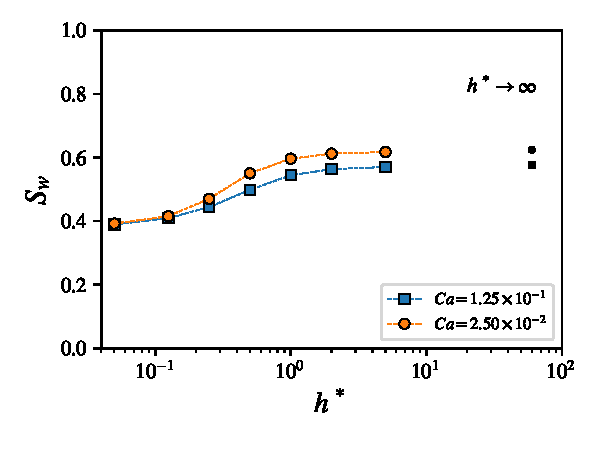
\includegraphics[scale=0.8]{RESULTS_saturation.pdf}
\caption{Saturation in wetting fluid as a function of the dimensionless gap between the plates.}
\end{figure}
\end{frame}


\begin{frame}[label={sec:org98afb82}]{Results: fluid-fluid interface}
\end{frame}

\begin{frame}[label={sec:orgb51f6ba}]{Results: solid-fluid drag force (1)}
\begin{figure}
\centering
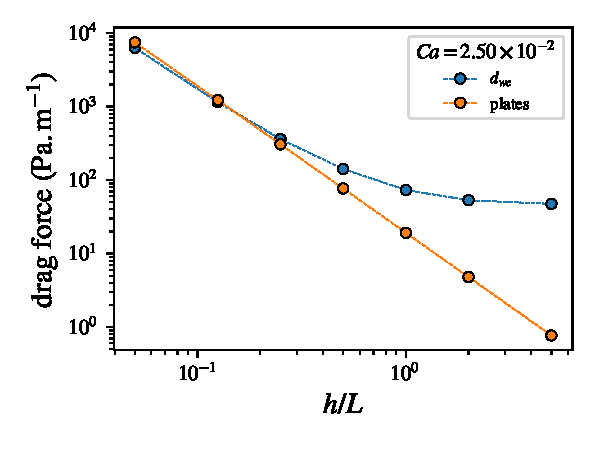
\includegraphics[scale=0.8]{RESULTS_drag.pdf}
\caption{Comparison of the solid-fluid drag upon the wedge and upon the Hele-Shaw plates as a function of the
dimensionless gap.}
\end{figure}
\end{frame}

\begin{frame}[label={sec:orgeed5a19}]{Results: solid-fluid drag force (2)}
\begin{alertblock}{Drag upon the plates}
\begin{enumerate}
\item constant inlet velocity whereas the gap between the plates is narrowing
\item drag : $-\mu_i \langle u_i \rangle \frac{12}{h^2}$
\item the drag upon the plates scales as $h^{-2}$
\end{enumerate}
\end{alertblock}

\begin{exampleblock}{Drag upon the wedge}

\begin{enumerate}
\item constant geometry
\item velocity gradient depends on the fluid-fluid interface position
\item pressure increases as the gap is narrowing
\end{enumerate}

\end{exampleblock}
\end{frame}



\begin{frame}[label={sec:org75b4b07}]{Results: fluid-fluid drag force (1)}
\begin{alertblock}{Fluid-fluid drag}
\begin{enumerate}
\item interface is changing (slightly)
\item pressure gradient increases as the gap is narrowing since the inlet velocity is constant
\end{enumerate}
\end{alertblock}
\end{frame}

\begin{frame}[label={sec:org76545b5}]{Results: fluid-fluid drag force (2)}
\end{frame}
\begin{frame}[label={sec:orgfc92227}]{Results: drag ratio}
\begin{figure}
\centering
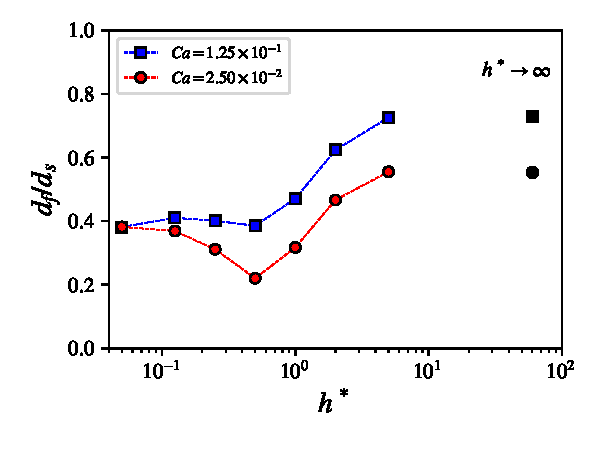
\includegraphics[scale=0.8]{RESULTS_dragRatio.pdf}
\caption{Ratio of fluid-fluid drag over solid-fluid drag as a function of the dimensionless gap
 between the plates.}
\end{figure}
\end{frame}

\begin{frame}[label={sec:orgbc5cfbd}]{Results: drag}
\begin{figure}
\centering
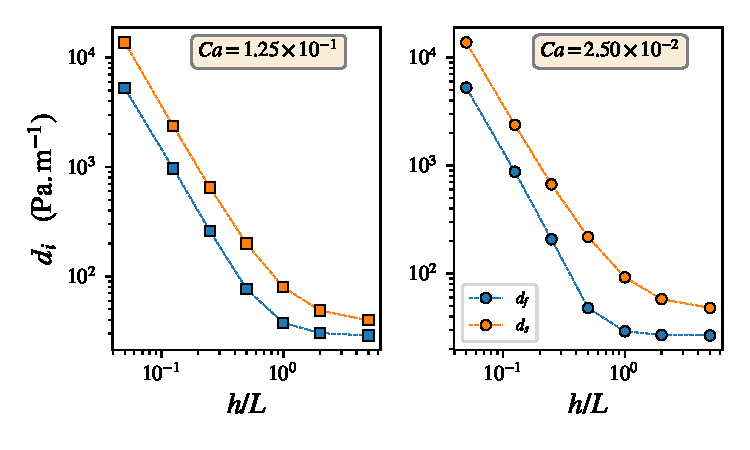
\includegraphics[scale=0.8]{RESULTS_dragSepare.pdf}
\caption{Comparison of fluid-fluid and solid-fluid drag force for differrent capillary numbers as a
function of the dimensionless gap.}
\end{figure}
\end{frame}

\begin{frame}[label={sec:orgab07557}]{Results: Flat interface}
What happens if the fluid-fluid interface is flat for \(1<h/L\)?

\begin{enumerate}
	\item we keep the drag upon the plates in the momentum transport equations
	\item the contact angle is 0 and the pressure jump across the interface is only due to the $x-y$ curvature
\end{enumerate}
\end{frame}

\begin{frame}[label={sec:org497bd82}]{Results: Dynamic film formation}
By following \cite{park1984two}, the thickness of the wetting fluid film
scales, at leading order, as 
\begin{equation}
\frac{h}{6}
\end{equation}

for \(Ca= 1.25 \times 10^{-1}\).
\end{frame}

\begin{frame}[label={sec:org00a4ea3}]{References}
\bibliographystyle{unsrt}
\bibliography{article}
\end{frame}
\end{document}